\documentclass[10pt,a4paper]{article}

\usepackage[margin=2cm]{geometry}
\usepackage[T1]{fontenc}
\usepackage{lmodern}
\usepackage{graphicx}
\usepackage{booktabs}
\usepackage{tabularx}
\usepackage{subcaption}
\usepackage{amsmath}
\usepackage{enumitem}
\usepackage{xcolor}
\usepackage[hidelinks]{hyperref}

\graphicspath{{../q1_mapreduce/plots/}}
\setlist{nosep,leftmargin=*}
\setlength{\parskip}{4pt}
\setlength{\parindent}{0pt}
\newcommand{\code}[1]{\texttt{#1}}
\renewcommand{\topfraction}{0.9}
\renewcommand{\bottomfraction}{0.8}
\renewcommand{\textfraction}{0.1}
\renewcommand{\floatpagefraction}{0.85}

\title{Distributed Systems HW3 -- Section 2\\
\large Weather Data Analytics (HW2 Q8) using MapReduce and gRPC}
\author{Team \textcolor{red}{XX}: Rajai Tarun Kanaiyalal (\textcolor{red}{roll no.}) \and \textcolor{red}{Teammate name (roll no.)}}
\date{}

\begin{document}
\maketitle

%=====================================================================
\section{Q1: Batch analytics using MapReduce}

In HW2 we solved the weather analytics problem (Q8) with a sequential program and with MPI. Here we solve the same problem,
with the same input and output, using MapReduce, and then compare it with our MPI program. The code and the full run
instructions are in \code{q1\_mapreduce/README.md}.

\subsection{How we ran it}
The assignment asks for Hadoop Streaming. Hadoop is not installed on the RCE cluster (there is no Hadoop module), and the
course told us to use a Slurm script until it is fixed. So we wrote the mapper, combiner and reducer as normal C++ programs
that read from stdin and write \code{key<TAB>value} lines to stdout. This is exactly what Hadoop Streaming expects, so the same
programs will also run on Hadoop without any change. Our Slurm script does the same steps that Hadoop would do:

\begin{enumerate}
\item \textbf{Split}: cut the input file into $P$ pieces (one per mapper).
\item \textbf{Map}: $P$ tasks run in parallel, each doing \code{mapper | sort | combiner} on its own piece.
\item \textbf{Shuffle}: the master merges all the sorted combiner outputs into one sorted file.
\item \textbf{Reduce}: one reducer reads that file and prints the final answer.
\end{enumerate}

\subsection{Our MapReduce design}
For every record, the mapper prints three lines, using these keys:

\begin{center}\small
\begin{tabular}{lll}
\toprule
Key & Value & How two values are combined \\
\midrule
\code{G} & count, sums, min/max, extreme count, hottest, coldest & add, min/max, hotter/colder \\
\code{S<station>} & count, temperature sum, rainfall sum & add \\
\code{I<interval>} & count (interval = timestamp / 60) & add \\
\code{K} & the $K$ from the header line & keep \\
\bottomrule
\end{tabular}
\end{center}

The main idea: \textbf{one record is treated as a small partial result with count 1}. So the mapper output, the combiner
input and the combiner output all have the same format, and the combiner and reducer only need to know how to merge two
lines with the same key. Since the merges are just additions, mins and maxes, the order does not matter. The answer is the
same no matter how the input is split or how many times the combiner runs. We never merge averages, only sums and counts,
and divide at the very end.

Top-$K$ stations and the busiest interval can only be decided after \emph{all} the counts are merged (the same bug we found in
HW2 when each process kept its own top-$K$). That is why we use \textbf{one reducer}: it sees every station and every interval.

\subsection{Important decisions}
Table~\ref{tab:decisions} lists the main decisions we took, why, and what effect we measured.

\begin{table}[!htbp]
\centering\small
\begin{tabularx}{\textwidth}{>{\raggedright\arraybackslash}p{3.8cm}>{\raggedright\arraybackslash}X>{\raggedright\arraybackslash}p{4.2cm}}
\toprule
Decision & Why & Effect \\
\midrule
Use a combiner & The mapper prints 3 lines per record, and the same keys repeat a lot inside one piece. & 10M records: 30M $\to$ 7M lines sent to the reducer; 52\,s $\to$ 16\,s. \\
Only one reducer & Top-$K$ and busiest interval need all the data in one place. & Reducer takes only 0.5--3.3\,s. \\
Mapper prints the numbers exactly as read & Printing them as doubles turned \code{24.49} into \code{24.489999999999998}. & Mapper output 2.1$\times$ smaller. \\
Read numbers with \code{strtod} & \code{stringstream} was very slow for millions of lines. & Combiner 2.9$\times$ faster. \\
\code{LC\_ALL=C sort} & The normal \code{sort} can ignore the tab and mix up keys like \code{S1} and \code{S10}. & Correct grouping. \\
Pipe \code{mapper|sort|combiner} & The full mapper output for 50M records is 7.5\,GB, but our disk quota is 10\,GB. & Nothing big is written to disk. \\
Same data, same node as MPI & A fair comparison with HW2. & Differences come from the model, not the setup. \\
\bottomrule
\end{tabularx}
\caption{Main design decisions.}
\label{tab:decisions}
\end{table}

\subsection{Correctness}
\begin{itemize}
\item \textbf{Local tests (69, all pass)}: the 9 HW2 test cases with expected outputs (ties, extreme values, $K>S$, $N=0$) give
the exact expected output. All 13 HW2 inputs plus generated 100K and 1M inputs, each split into 1, 2, 4 and 8 pieces, give the
same output as the HW2 sequential program.
\item \textbf{Cluster}: the same output as sequential on one node and on two nodes, and all 44 benchmark runs are correct.
\end{itemize}

\textbf{One small rounding difference.} From 10M records onwards, the last digits of \code{TOTAL\_RAINFALL} differ, e.g.\
249966638.539998 (sequential) vs 249966638.540026 (MapReduce). The true value is 249966638.54, so both are slightly off.
A \code{double} only keeps about 15--16 digits, and adding 10 million numbers in a different order gives a slightly different
rounding. Our HW2 MPI program shows the same difference against sequential when it uses 1, 2 or 4 workers. So our checker
(\code{compare\_outputs.py}) requires counts, ids and timestamps to match exactly, and allows decimal numbers to differ only by a
relative $10^{-10}$. Every run passed: 15 matched exactly and 25 differed only by this rounding.

\subsection{Experimental setup}
We used the HW2 dataset generator with seed 42, $K=10$ and $S=100$, and input sizes of 1M, 10M, 20M and 50M records (50M
records is 2.1\,GB). We ran MPI with 1, 2, 4 and 8 workers and MapReduce with 1, 2, 4 and 8 mappers. All runs of one benchmark
were in the same Slurm job, on one node, on the same data. We measured the total time of each run (including reading the input),
the time of each MapReduce stage, and the peak memory of every process.

\subsection{Results}

\begin{figure}[!htbp]
\centering
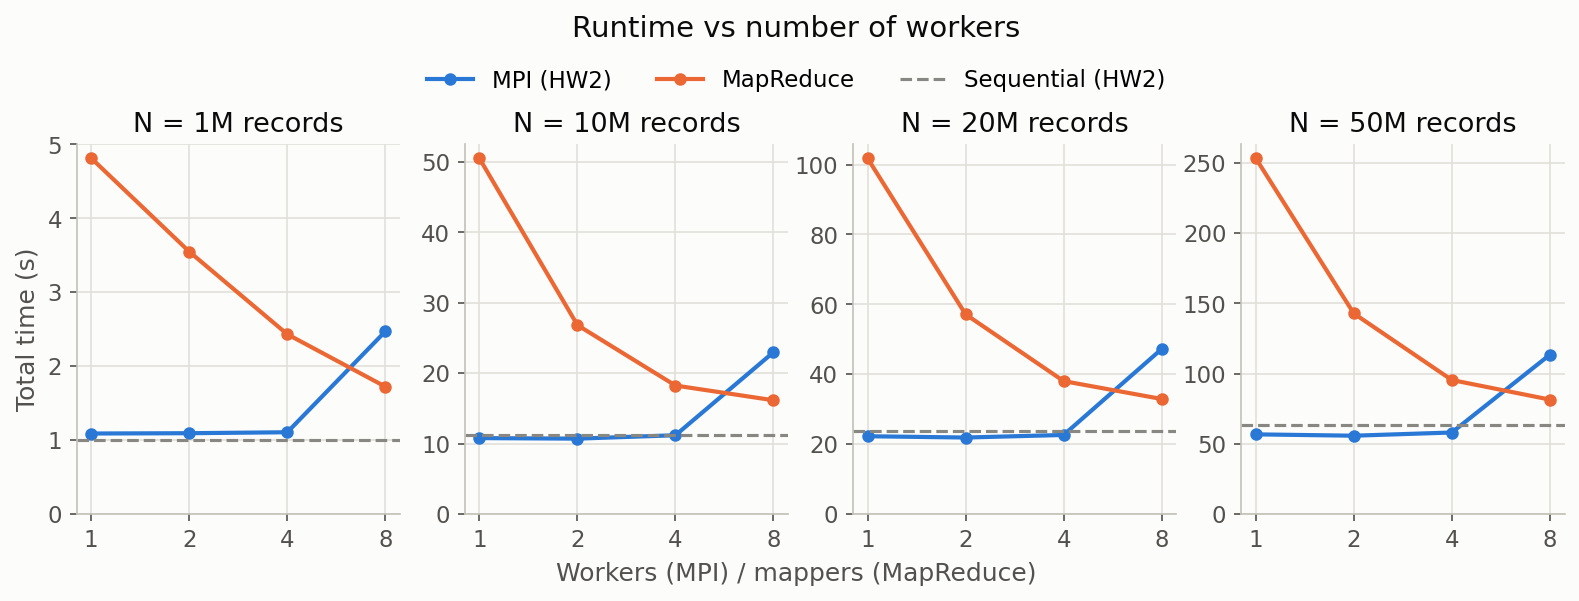
\includegraphics[width=\textwidth]{runtime_vs_workers.png}
\caption{Total time vs number of workers/mappers. Dashed line: HW2 sequential.}
\label{fig:rt}
\end{figure}

\begin{table}[!htbp]
\centering\small
\begin{tabular}{rrrrrrrrrr}
\toprule
$N$ & Seq & MPI 1 & MPI 2 & MPI 4 & MPI 8 & MR 1 & MR 2 & MR 4 & MR 8 \\
\midrule
1M  & 1.00  & 1.09  & 1.09  & 1.11  & 2.47   & 4.81   & 3.55   & 2.43  & 1.72 \\
10M & 11.22 & 10.78 & 10.70 & 11.19 & 22.98  & 50.51  & 26.83  & 18.24 & 16.16 \\
20M & 23.87 & 22.25 & 21.88 & 22.61 & 47.21  & 101.77 & 57.13  & 38.03 & 32.91 \\
50M & 63.65 & 56.74 & 55.78 & 58.06 & 113.48 & 253.44 & 142.90 & 95.46 & 81.50 \\
\bottomrule
\end{tabular}
\caption{Total time in seconds (MR = MapReduce).}
\label{tab:rt}
\end{table}

\paragraph{MPI is faster overall (Fig.~\ref{fig:rt}, Table~\ref{tab:rt}).}
At 50M records the best MPI run takes 55.8\,s and the best MapReduce run takes 81.5\,s. Both grow linearly with the input size.
MapReduce does much more work per record. MPI reads each record once into a small binary struct and sends structs. MapReduce
turns each record into 3 text lines (151 bytes, 3.6 times bigger than the input), sorts all these lines, and then reads the
numbers back from text in the combiner. With only one mapper, MapReduce is 4 times slower than sequential (253\,s vs 64\,s).

\paragraph{MPI does not get faster with more workers.}
From our HW2 timing logs, at 50M records rank 0 spends about 46\,s of the 56\,s just \emph{reading the input file alone}. The
workers can only start after that, so adding more workers only speeds up the small compute part. With 8 workers the time even
doubles, and the HW2 log shows that it is rank 0's reading that becomes twice as slow. Our best guess is that the 8 waiting MPI
processes keep the CPUs busy while they wait, which slows down rank 0.

\begin{figure}[!htbp]
\centering
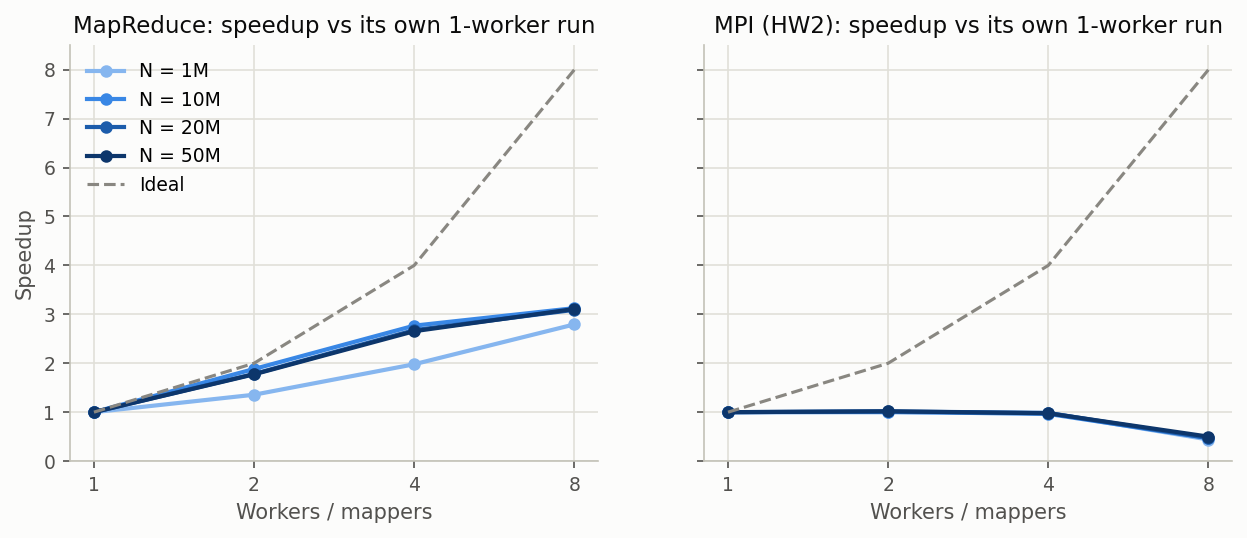
\includegraphics[width=0.85\textwidth]{speedup.png}
\caption{Speedup of each implementation compared with its own 1-worker run. Dashed line: ideal speedup.}
\label{fig:speedup}
\end{figure}

\paragraph{MapReduce gets faster with more mappers, but not 8 times faster (Fig.~\ref{fig:speedup}).}
In MapReduce each mapper reads and processes its own piece, so the slow part is done in parallel. At 50M records MapReduce is
3.1 times faster with 8 mappers than with 1. It does not reach 8 times because:
\begin{itemize}
\item \textbf{Splitting the input is done by one process} and always takes about 20\,s at 50M. That is 8\% of the time with 1
mapper but 24\% with 8 mappers. (In real Hadoop this step does not exist, because HDFS already stores the file in pieces.)
\item \textbf{Shuffle and reduce get slower with more mappers} (2\,s with 1 mapper, 9.5\,s with 8), because more mappers send
more lines to the reducer (explained below).
\item \textbf{All 8 mappers share one node}, so they compete for the same memory and disk.
\end{itemize}

\begin{figure}[!htbp]
\centering
\begin{subfigure}{0.49\textwidth}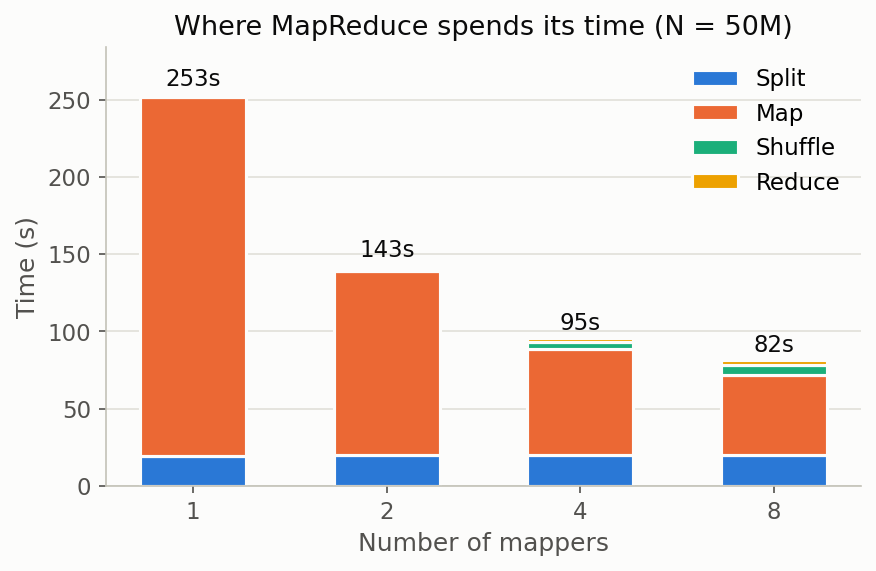
\includegraphics[width=\linewidth]{mr_stage_breakdown.png}\caption{Time of each stage, 50M records.}\label{fig:stages50}\end{subfigure}\hfill
\begin{subfigure}{0.49\textwidth}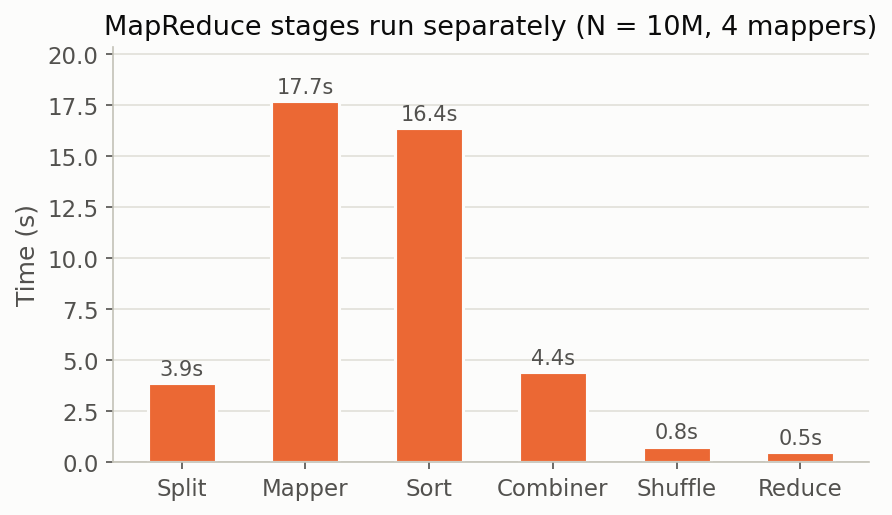
\includegraphics[width=\linewidth]{map_phase_stages.png}\caption{Map phase split into parts, 10M records, 4 mappers.}\label{fig:mapstages}\end{subfigure}
\caption{Where MapReduce spends its time.}
\end{figure}

\paragraph{Where the time goes (Fig.~\ref{fig:stages50}, \ref{fig:mapstages}).}
The map phase (mapper + sort + combiner) takes almost all the time: 232 of 253\,s with 1 mapper at 50M. To see what is inside
it, we also ran the three parts separately (10M records, 4 mappers): the mapper took 17.7\,s, the sort 16.4\,s and the combiner
only 4.4\,s. So most of the time is spent on \textbf{converting records to text and sorting them}, not on the actual
analytics. The mapper is slow because it splits every line into words and writes 1.5\,GB of text for 10M records.

\begin{figure}[!htbp]
\centering
\begin{subfigure}{0.52\textwidth}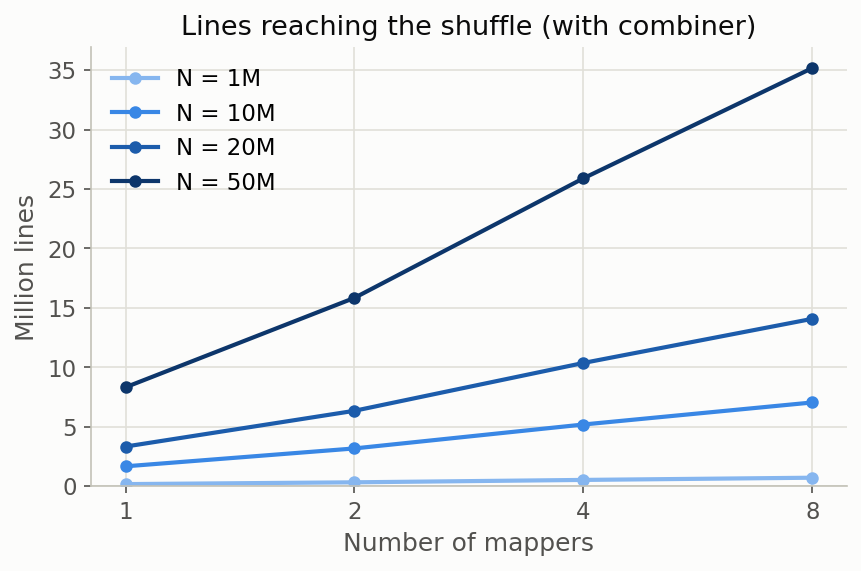
\includegraphics[width=\linewidth]{shuffle_lines.png}\caption{Lines sent to the reducer.}\label{fig:shuffle}\end{subfigure}\hfill
\begin{subfigure}{0.46\textwidth}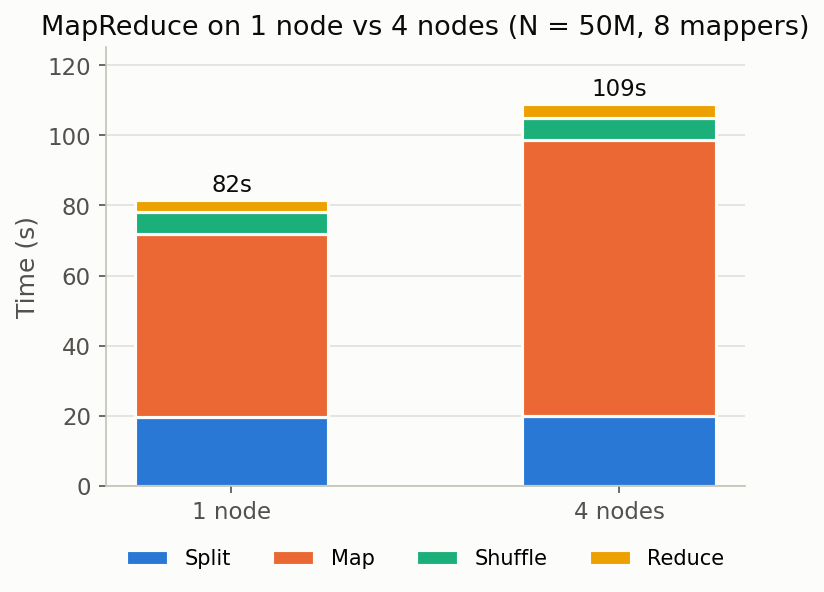
\includegraphics[width=\linewidth]{multinode.png}\caption{1 node vs 4 nodes, 50M records, 8 mappers.}\label{fig:multinode}\end{subfigure}
\caption{Data sent to the reducer, and running on more nodes.}
\end{figure}

\paragraph{More mappers send more data to the reducer (Fig.~\ref{fig:shuffle}).}
With 1 mapper at 50M, 8.3M lines reach the reducer; with 8 mappers, 35.2M lines. The reason: each mapper's combiner can only
merge the lines of its \emph{own} piece. If the records of one interval are spread over 5 pieces, that interval is sent 5 times.
Almost all of these lines are interval lines: there are about 8.3M intervals with only about 6 records each, so they get spread
over many pieces. We checked this with a simple formula: an interval with on average 6 records, split randomly over $P$ pieces,
appears in $P(1-e^{-6/P})$ pieces. This predicts 8.31M, 15.84M, 25.90M and 35.18M lines for 1, 2, 4 and 8 mappers, which matches
our measurements.

\begin{figure}[!htbp]
\centering
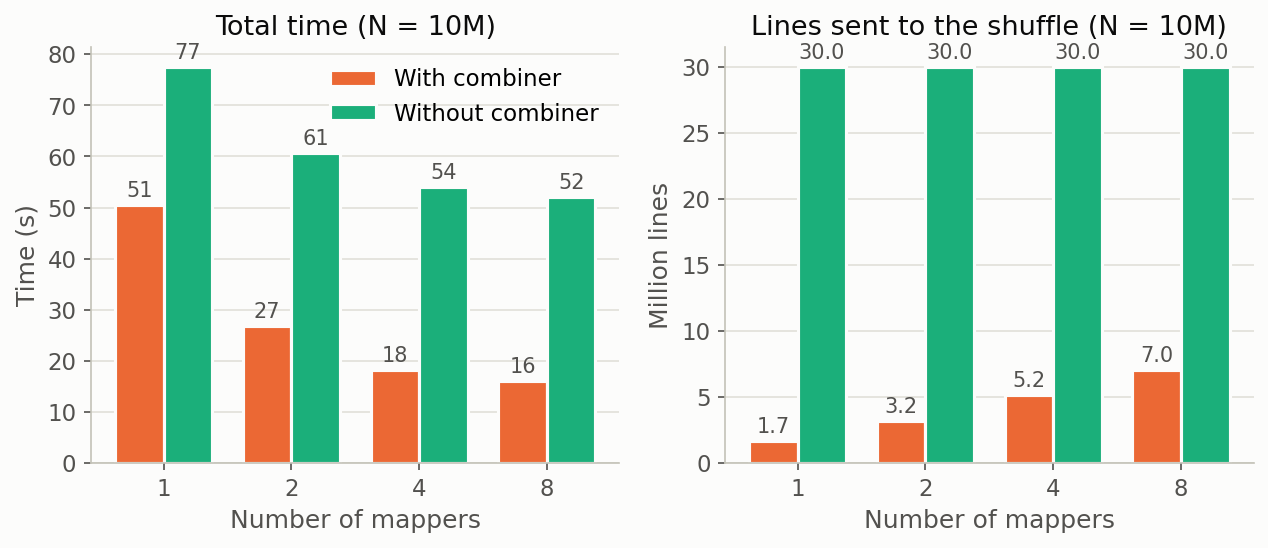
\includegraphics[width=0.85\textwidth]{combiner_effect.png}
\caption{MapReduce with and without the combiner, 10M records.}
\label{fig:comb}
\end{figure}

\paragraph{The combiner makes a big difference (Fig.~\ref{fig:comb}).}
Without the combiner, all 3 lines of every record go to the one reducer: 30M lines at 10M records. The shuffle then takes
about 15\,s and the reducer 13\,s, instead of less than 1.3\,s each. With 8 mappers the whole run is 3.2 times faster with the
combiner (16\,s vs 52\,s). Without it, adding mappers barely helps, because the single reducer becomes the bottleneck.

\begin{figure}[!htbp]
\centering
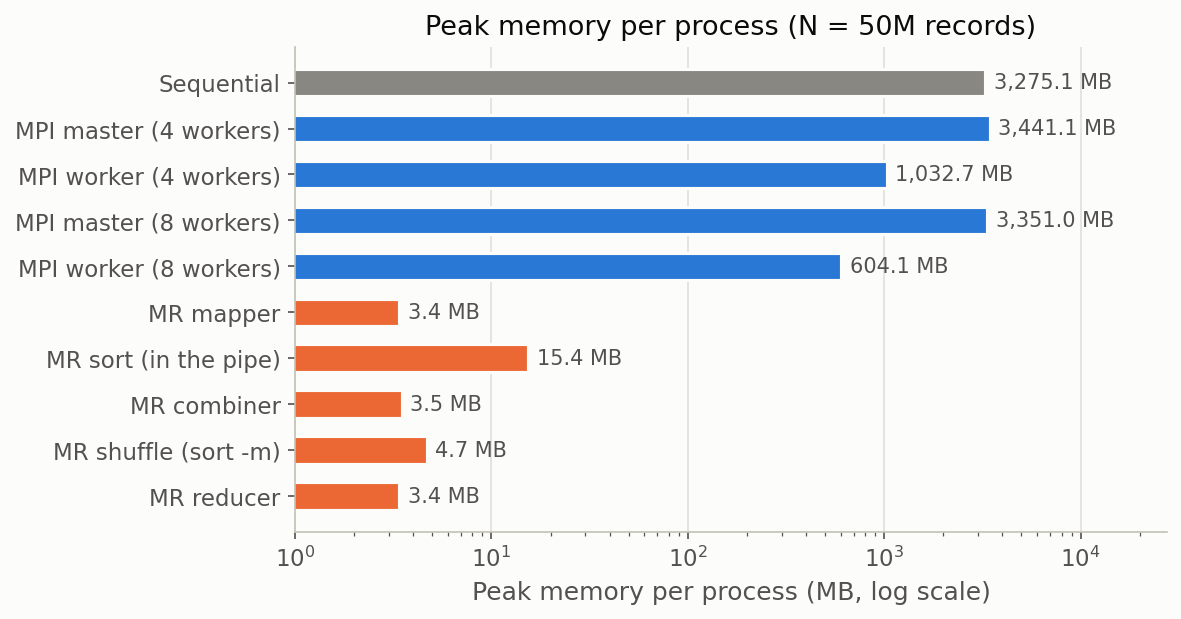
\includegraphics[width=0.68\textwidth]{memory.png}
\caption{Peak memory of each process, 50M records (log scale).}
\label{fig:mem}
\end{figure}

\paragraph{MapReduce uses much less memory (Fig.~\ref{fig:mem}).}
This is where MapReduce clearly wins. In MPI, rank 0 reads \emph{all} the records into memory before sending them out: 50M
records $\times$ 56 bytes is about 2.8\,GB, plus the hash map of all the intervals. So rank 0 used 3.4\,GB and each worker
around 1\,GB, which is 7.6\,GB for the whole run with 4 workers. Our MapReduce programs only look at one line at a time: the
mapper, combiner and reducer each used about 3.5\,MB, and \code{sort} used about 15\,MB (it writes to temporary files on disk when
needed). The whole MapReduce run used only 91\,MB, about \textbf{80 times less}. This means MPI cannot handle data bigger than
one machine's memory, while MapReduce can.

\paragraph{Running on 4 nodes was slower (Fig.~\ref{fig:multinode}).}
We also spread the 8 mappers over 4 nodes. This made the run slower (82\,s $\to$ 109\,s); only the map phase got slower. Our
explanation: the input pieces are stored in our home folder, which is a shared network drive. On one node, the pieces were
just written by the same node and are still in its memory, so reading them is fast. On 4 nodes, the other 3 nodes must download
their pieces over the network at the same time. Real Hadoop avoids this with HDFS: the pieces are stored on the worker nodes'
own disks, and each map task runs on the node that already has its piece (\emph{data locality}).

\subsection{MPI vs MapReduce: summary}
\begin{center}\small
\begin{tabularx}{\textwidth}{>{\raggedright\arraybackslash}p{3cm}>{\raggedright\arraybackslash}X>{\raggedright\arraybackslash}X}
\toprule
 & MPI (HW2) & MapReduce \\
\midrule
Time at 50M (best) & \textbf{55.8\,s} & 81.5\,s \\
Speedup, 1 $\to$ 8 workers & none (rank 0 reads the input alone) & \textbf{3.1$\times$} \\
Memory at 50M & 7.6\,GB (3.4\,GB on rank 0) & \textbf{91\,MB} \\
Data sent & binary structs & text lines, reduced by the combiner \\
Code we had to write & custom MPI datatype, scatter, 9 different send/receive messages, merging & 3 small programs, no communication code \\
Adding a new statistic & change the struct, the messages and the merge & add one new key \\
If a process crashes & the whole job fails & Hadoop re-runs only that task \\
\bottomrule
\end{tabularx}
\end{center}

\textbf{Conclusion.} For our 2\,GB input on one machine, MPI is faster because it works on binary data in memory. MapReduce
is slower because of all the text conversion and sorting, but it gets faster with more mappers, uses 80 times less memory, and
was much simpler to write. For data that does not fit on one machine, MapReduce is the better choice.

%=====================================================================
\section{Q2: Real-time streaming analytics using gRPC}
\textit{To be added.}

\end{document}
